\documentclass{article}

\renewcommand{\familydefault}{\sfdefault}  %serifenlose Schrift
\usepackage{helvet} % Schrift: Helvetica


\usepackage{graphicx,graphics,tikz}
\usepackage{amsmath}
\usepackage{amsthm}
\usepackage{amsfonts}
\usepackage{amssymb}
\usepackage{marvosym} % to be able to show male and female symbols with: \Female and \Male
\usepackage{gensymb}
\usepackage[graphics,tightpage,active]{preview}
\PreviewEnvironment{tikzpicture}
\newlength\imagewidth
\newlength\imagescale

\begin{document}

%\pgfmathsetlength{\imagewidth}{10cm} % desired displayed width of image
%\pgfmathsetlength{\imagescale}{\imagewidth/2000} % pixel width of image
% adjust scale of tikzpicture (and direction of y) such that pixel
% coordinates can be used for drawing overlays:
\usetikzlibrary{backgrounds}

\begin{tikzpicture}[scale=1.51]%[x=\imagescale,y=-\imagescale]
\node[anchor=north west,inner sep=0pt,outer sep=0pt,scale=1] at (3.5,0) {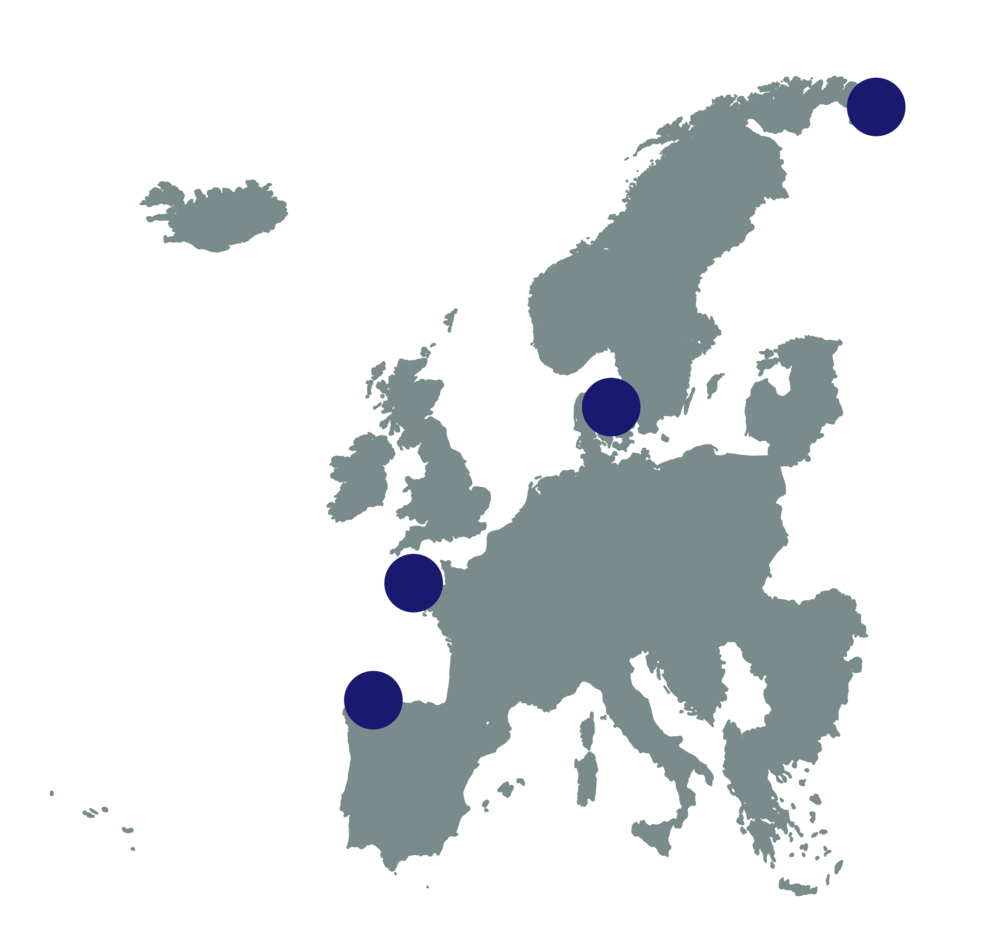
\includegraphics[width=5cm]{OnlySamples_r.png}};

\begin{scope}[xshift=1.5cm,yshift=0.5cm]


\draw [color=black](5,-1.25+0.8) node {\small{Norway}};
\draw [color=black](3.7-1,-1.85) node {\small{Denmark}};
\draw [color=black](3.58-0.7,-2.43) node {\small{Brittany}};
\draw [color=black](3.4-0.7,-2.82) node  {\small{Spain}};

\node (Norway) at (4.9,-0.85cm) {};
\node (Denmark) at (4.03,-1.85cm) {};
\node (France) at (3.38,-2.43cm) {};
\node (Spain) at (3.23,-2.82cm) {};
\end{scope}

\node (Bodo) [anchor=west] at (5.3,-0.4) {Bod{\o}};
\draw [-latex] (Norway) to [out=180,in=270] (Bodo);
\draw [-latex] (Denmark) to [out=90,in=270] (Bodo);
\draw [-latex] (France) to [out=90,in=270] (Bodo);
\draw [-latex] (Spain) to [out=90,in=270] (Bodo);

\draw [color=black, fill=white] (0.5,-1.8) rectangle (3.56,0.7);
\node at (2,0.5) {Acclimation at 9\celsius};
\node[anchor=north west,inner sep=0pt,outer sep=0pt,scale=1] at (0.7,0.3) {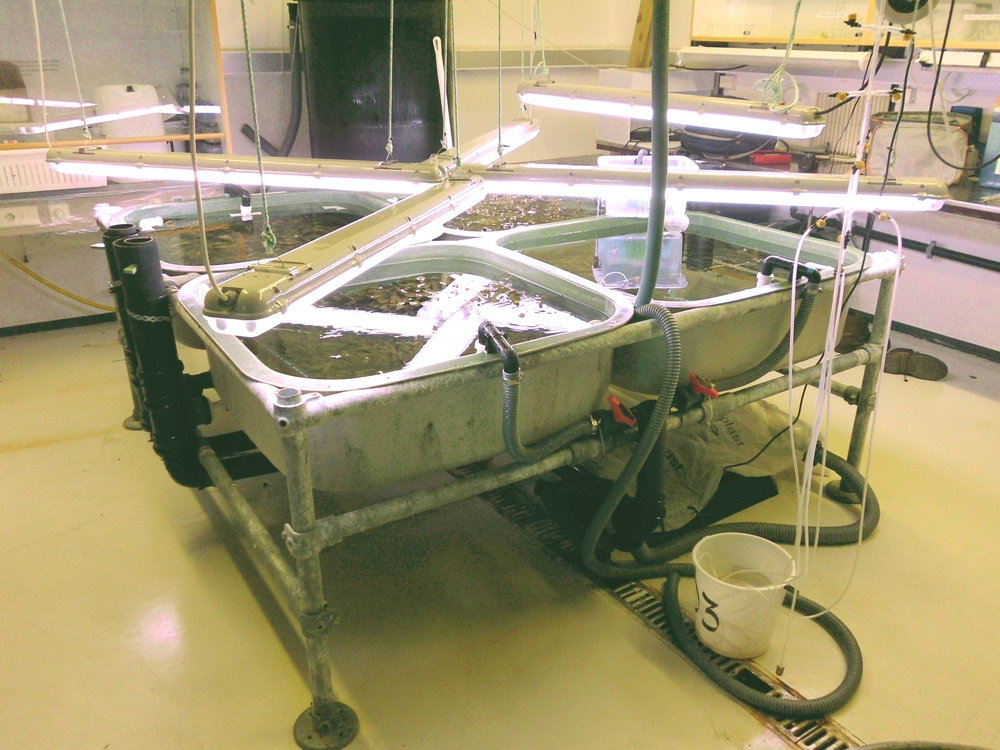
\includegraphics[width=4cm]{DSCI0153_new_r.JPG}};



\end{tikzpicture}

\end{document}